\documentclass[../main.tex]{subfiles}
\graphicspath{{\subfix{./}}}
\begin{document}
\everymath{\displaystyle}
%-------------------------------
\vspace{0.2in}
\hrule
\vspace{0.1in}
\section{MOSFET}
\hrule
\begin{xltabular}{\textwidth}{|X|X|}
	\hline
	\endhead
	\hline
	\endfoot
	\endlastfoot
	\underline{\textbf{Condensador MOS}}

	subindices: s = superficie silicio, ox = placa de óxido aislante
	\newline\newline
	$\begin{aligned}
			 & K_{\text{SiO}_2} = e_{ox} = 3.9                                      \\
			 & \phi_M =\chi +E_c - E_F                                              \\
			 & \phi_M =\phi_S                                                       \\
			 & \phi_{F_\text{Si-N}} = E_F - E_i = k_BT\ln(N_D/n_i)                  \\
			 & \phi_n = \text{debe medirse}                                         \\
			 & \phi_p = -60\ln(\frac{N_A}{n_i})\si{\mV}                             \\
			 & V_{FB} = - (\phi_{n^+} - \phi_p) =\phi_B = 2\phi_s = v_t\ln(N_A/n_i) \\
		\end{aligned}$
	\newline
	\textbf{límite de inversion}
	$$E_{i_\text{superficie}} - E_{i_\text{sustrato}} = 2(E_F - E_{i_\text{sustrato}})$$
	&
	\underline{\textbf{Parámetros Transistor MOSFET}}
	\begin{center}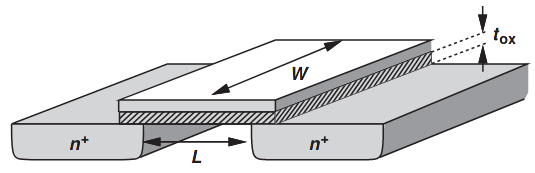
\includegraphics[scale=0.5]{assets/mosfet}\end{center}
	$$C_{ox}' = \frac{\varepsilon_0K_o}{\chi_o} = \frac{\varepsilon_0\varepsilon_{ox}}{t_{ox}}, [\si{\F\per\square\cm}]$$
	$$C_{ox} = \frac{\varepsilon_0 \varepsilon_{ox}}{t_{ox}}\cdot L\cdot W, \text{[\si{\F}]}$$
	$$V_{GB} = V_{GS}$$

	%-----------
	\\
	%--------------
	\begin{center}
		\begin{tabular}{|c|c|c|}
			\firsthline
			\multicolumn{3}{| c |}{\textbf{Para sustrato N}}
			\\
			\hline
			Estado      & $V_G$       & Concent. de portadores n \\
			\hline
			Acumulación & $> V_{FB}$  & $>N_D$                   \\
			Banda plana & $= V_{FB}$  & $=N_D$                   \\
			Vaciamiento & $< V_{FB}$  & $< N_D$                  \\
			Inversión   & $<< V_{FB}$ & $p > N_D$                \\
			\hline
		\end{tabular}\newline\newline\end{center}
	\textbf{Capacitancias}
	$$C_{ox} = \frac{\epsilon_0K_{ox}A_G}{\chi_{ox}}, ~~~~~ C_{ox_{\text{vac}}} =  \frac{C_{ox} C_s}{C_{ox} + C_s}$$
	\textbf{Relación $V_G$ $\phi_s$ (Si P en vaciamiento)}
	$$\chi_{ox} = t_{ox}$$
	$$V_G = \Delta\phi_s + \Delta\phi_{ox}$$
	$$V_G = \phi_s + \frac{K_s}{K_{ox}}\chi_{ox}\sqrt{\frac{2qN_A}{K_s\epsilon_{ox}}}$$

	&
	$$V_{ov} = \begin{cases} \text{NMOS: } V_{GS} - V_{TH}\\\text{PMOS: }V_{SG} - |V_{TH}| \end{cases}$$
	$$\text{coeff. mod. largo ch: } \lambda, ~~~ [\lambda] = \si{\per\V}$$
	$$\text{Parámetro del proceso } K' = \mu_nC_{ox}'$$
	$$\text{Transconductancia del proceso } K = \mu_nC_{ox}'\frac{W}{L}$$
	$$I_{D_0} = I_D\bigg|_{V_{ov}=0}\approx 0.1 \si{\micro\A}\cdot\frac{W}{L}$$
	$$\text{Pendiente subumbral}\begin{cases}
			S = \bigg[\frac{d}{dV_{GS}}\log(I_{DS})\bigg]^{-1} \\
			S = v_t\ln(10)\cdot m                              \\
			m=1+\frac{C_{dep}}{C_{ox}}\end{cases}$$
	\textbf{Valores en condiciones estándar}
	$$S(T=300)  = 60\si{\mV}/\text{década}$$
	$$S(T=273,15) = 80\si{\mV}/\text{década}$$
	\\
	\hline
	\underline{\textbf{N-channel MOSFET}}
	$$\text{Subumbral} \begin{cases}
			V_{ov} < 0 \\
			I_D = I_{D_0}\exp\bigg(\frac{V_{ov}}{S}\ln(10)\bigg)
		\end{cases}$$
	$$\text{Triodo-lineal}\begin{cases}
			V_{ov} > 0                                           \\
			V_{DS} < V_{ov}                                      \\
			I_D = K\bigg(V_{ov}V_{DS} -\frac{1}{2}V_{DS}^2\bigg) \\
			R_{ch} = \frac{V_{DS}}{I_D} = (KV_{ov})^{-1}         \\
		\end{cases}$$
	$$\text{Saturación}\begin{cases}
			V_{ov} > 0                                              \\
			V_{DS} > V_{ov}                                         \\
			I_D = \bigg(\frac{K}{2}V_{ov}^2\bigg)(1+\lambda V_{DS}) \\
		\end{cases}$$
	$$g_m = \frac{\partial I_D}{\partial V_{GS}}\bigg|_Q = KV_{ov} = \frac{2I_D}{V_{ov}} = \sqrt{2KI_D}$$
	&
	\underline{\textbf{P-channel MOSFET}}
	$$\text{Subumbral} \begin{cases}
			V_{ov} < 0 \\
			I_D = I_{D_0}\exp\bigg(\frac{V_{ov}}{S}\ln(10)\bigg)
		\end{cases}$$
	$$\text{Triodo-lineal}\begin{cases}
			V_{ov} > 0                                            \\
			V_{SD} < V_{ov}                                       \\
			I_D = K\bigg(V_{ov}V_{SD} - \frac{1}{2}V_{SD}^2\bigg) \\
			R_{ch} = \frac{V_{DS}}{I_D} = (KV_{ov})^{-1}          \\
		\end{cases}$$
	$$\text{Saturación}\begin{cases}
			V_{ov} > 0                                              \\
			V_{SD} > V_{ov}                                         \\
			I_D = \bigg(\frac{K}{2}V_{ov}^2\bigg)(1+\lambda V_{SD}) \\
		\end{cases}$$
	$$g_m = \frac{\partial I_D}{\partial V_{SG}}\bigg|_Q = KV_{ov} = \frac{2I_D}{V_{ov}} = \sqrt{2KI_D}$$
	\\
	\hline

	\begin{center}
		\begin{tabular}{|l|c|c|c|}
			\firsthline
			\multicolumn{4}{|c|}{\textbf{Capacitancias parásitas}}                     \\
			\hline
			Región de operación & $C_{GD}$            & $C_{GB}$ & $C_{GS}$            \\
			\hline
			                    &                     &          &                     \\
			Subumbral           & $C_{OV}$            & $C_{OX}$ & $C_{OV}$            \\
			                    &                     &          &                     \\
			\hline
			                    &                     &          &                     \\
			Triodo              & $\frac{1}{2}C_{OX}$ & $C_{OX}$ & $\frac{1}{2}C_{OX}$ \\
			                    &                     &          &                     \\
			\hline
			                    &                     &          &                     \\
			Saturación          & $C_{OV}$            & $C_{OX}$ & $\frac{2}{3}C_{OX}$ \\
			                    &                     &          &                     \\
			\hline
		\end{tabular}\end{center}
	&
	\underline{\textbf{Modelo Digital del MOSFET}}
	\begin{itemize}
		\item $V_{DD} = 1, GND = 0$
		\item Entrada: $t_{rise}, t_{fall}$
		\item Salida: $t_{HL}, t_{LH}  = 0.7 RC$
		\item $V_o > 0.9 V_{DD} \implies 1$
		\item $V_o < 0.1 V_{DD} \implies 0$
		\item $0.1 V_{DD} < V_o < 0.9 V_{DD} \implies ?$
		\item CMOS: Uso NMOS y PMOS para evitar pérdida de potencia
	\end{itemize}
	\\
	\hline
	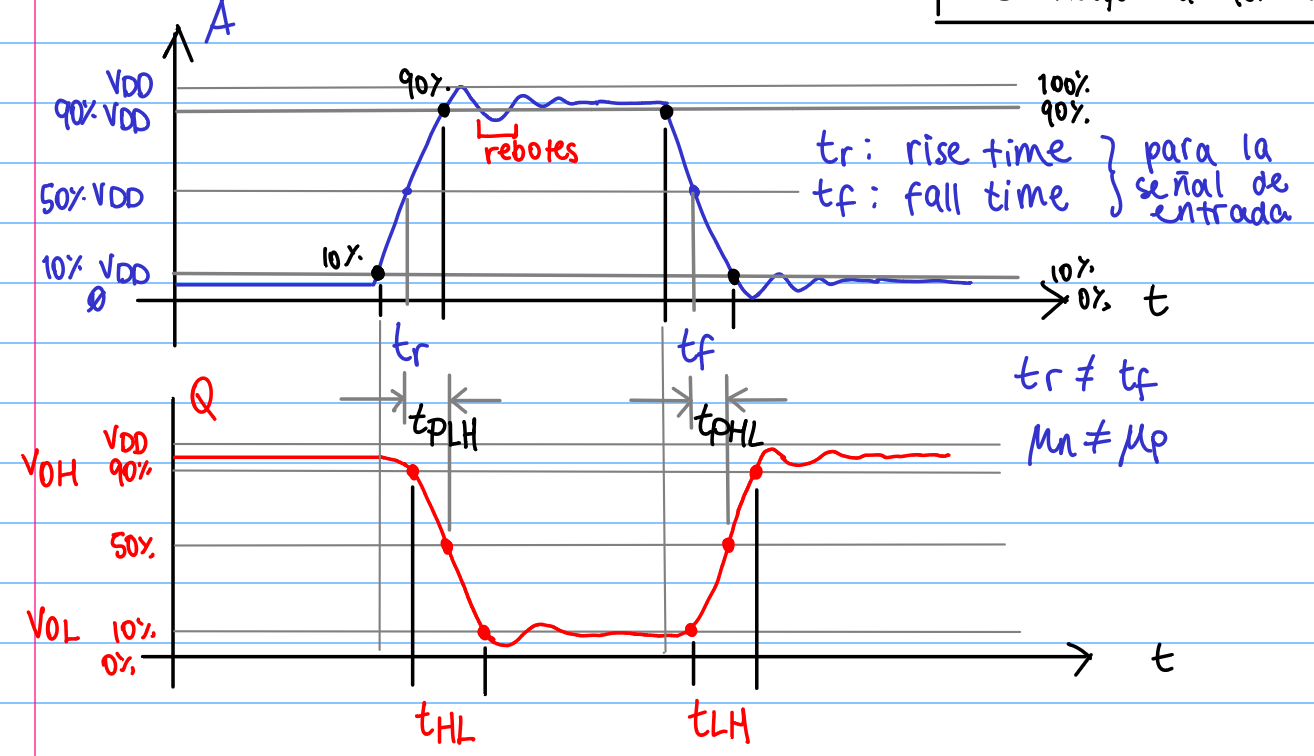
\includegraphics[scale=0.35]{assets/digital-timings}
	&
	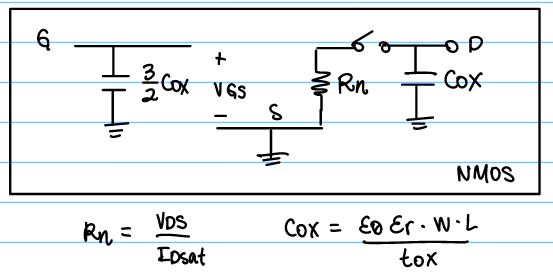
\includegraphics[scale=0.5]{assets/digital-model}
	\\
	\hline
	\multicolumn{2}{|c|}{\textbf{Aplicaciones digitales}}
	\\
	\hline
	\textbf{Compuerta de transmisión}\newline
	$$t_{delay} = 0.7 R_nC_{tot} = 0.7 R_n (C_L + \frac{C_{ox}}{2})$$
	\newline
	\textbf{Oscilador de anillo}: Conexión recursiva de compuertas not
	$$f_{osc} = \frac{1}{n(t_{PHL} + t_{PLH})}$$
	Capacitancia en cualquier nodo:
	$$C_{tot} = C_{in} + C_{out}$$
	&
	\underline{\textbf{Inversor CMOS}}\newline
	\textbf{Potencia estática del inversor}
	Fugas ($10^{-13}$ cada una):\newline
	+ corriente subumbral
	+ fuga de compuerta(desgaste óxido)
	+ corriente en reversa unión PN \newline
	\textbf{Potencia dinámica del inversor}\newline
	$$P_{SC} = I_{SC} V_{DD} = \frac{2}{3}K\frac{t_r}{T}\left(\frac{V_{DD}}{2} - V_{TH}\right)$$
	Con carga capacitiva: $P_L = AfC_LV_{DD}^2$\newline

	A es factor de actividad = probabilidad de que var[ien los datos


	\\
	\hline
\end{xltabular}
%----------------------------------------
\end{document}